\subsection{Die Datenbank}

Das in unserem System verwendete Datenbank-Management-System ist \emph{Postgres}. Es läuft in einem eigenen \emph{Docker}-Container. Als Datenbankschnittstelle verwendeten wir das ORM \emph{peewee}, welches Tabellen einer relationalen Datenbank auf sogenannte Modell-Klassen abbildet. Da jede unserer Modell-Klassen weitere Funktionalität benötigt, haben wir eine abstrakte Modell-Klasse (\code{BaseModel}) definiert, welche als Superklasse für jede weitere Modellklasse dient, und welche selbst von \code{peewee.Model} erbt, wie in \autoref{fig:database-class} zu erkennen ist. Diese Funktionalitäten sind
\begin{itemize}
	\item die explizite Definition eines Primärschlüssels (\code{id}) mit dem Typ einer Zeichenkette, welcher einen \emph{Universally unique identifier} (UUID) enthält,
	\item Daten, wann ein Objekt erzeugt und wann es zuletzt aktualisiert wurde
	\item und einen menschen-lesbaren Bezeichner (\code{readable\_id}), welcher prozedural erzeugt wird und einer verbesserten Nutzerinteraktion dient.
\end{itemize}
Weiterhin wurde die Methode \code{save} überschrieben aus \code{peewee.Model} überschrieben, um darin den Feldern \code{created\_at}, \code{updated\_at} und \code{readable\_id} ihre Werte zuzuweisen.

\begin{figure}[!ht]
	\centering
	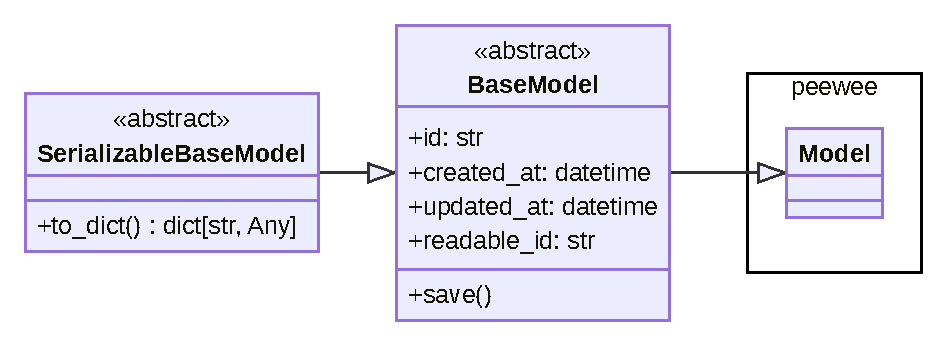
\includegraphics[width=0.75\linewidth]{images/diagrams/database-class.pdf}
	\caption{Klassendiagramm der abstrakten Modell-Klassen des ORM. \code{BaseModel} erbt von \code{peewee.Model}, um weitere Funktionalität hinzuzufügen. Dazu gehören Felder für \code{datetime}-Objekte, welche angeben, wann das Objekt erstellt und aktualisiert wurde. Weiterhin besitzt jedes Objekt eine \code{readable\_id}, welche die Identifizierung durch einen Menschen vereinfachen soll. Davon erbt \code{SerializableBaseModel}, um die Serialisierung von Objekten zu ermöglichen.}
	\label{fig:database-class}
\end{figure}

Von \code{BaseModel} erbt \code{SerializableBaseModel}, welches die zusätzliche Methode \code{to\_dict} implementiert. Damit lässt sich das Objekt JSON-serialisieren, um es bei Bedarf an das Frontend der Anwendung senden zu können.

\begin{figure}[!ht]
	\centering
	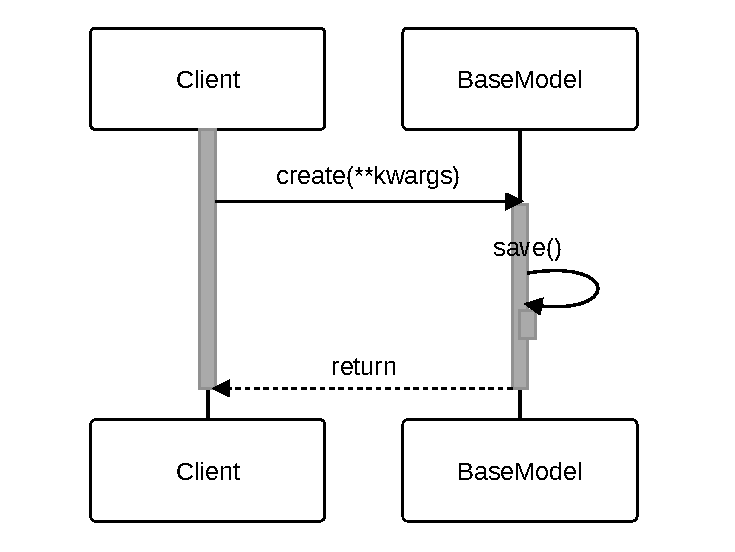
\includegraphics[width=0.75\linewidth]{images/diagrams/database-seq.pdf}
	\caption{Sequenzdiagramm der Erstellung eines Objektes über die Methode \code{create}. In \code{create} wird sowohl das Objekt initialisiert, als auch Selbstaufruf von \code{save} in der Datenbank abgelegt.}
	\label{fig:database-seq}
\end{figure}

Da die hinzugefügten Funktionalitäten in der überschriebenen Methode \code{save} implementiert wurden, sind diese gut in das Modell-System von \emph{peewee} integriert. Da \code{save} auch in \code{create} aufgerufen wird, wie in \autoref{fig:database-seq} zu erkennen, ist die Funktionalität damit automatisch auch bei der direkten Erzeugung eines neuen Objekts gegeben.

Alle im Rahmen unseres Projektes definierten Modell-Klassen erben von \code{BaseModel} oder \code{SerializableBaseModel} und erhalten damit die hinzugefügten Attribute.